% ============================================================================
%  ECE 431 -- Sheet 1 Solutions
%  Style: sheet-answering-style.md
% ============================================================================

\begin{question}[Question 1]The equation of motion of a one-dimensional electron oscillator due to an
electric field $e(t)$ is
\begin{equation*}
  \frac{\partial^{2}x}{\partial t^{2}}
  + \sigma\frac{\partial x}{\partial t}
  + \frac{k}{m}\,x(t)
  = -\frac{e}{m}\,e(t)
\end{equation*}
where $x(t)$ is the excursion from the equilibrium position, $\sigma$, $k$, and $m$ are,
respectively, the damping constant, the restoring (``spring constant'') coefficient, and electron
mass. The charge is $-e$.

\begin{enumerate}[label=(\Alph*)]

  \item If $e(t)=\mathrm{Re}[E\,\exp(j2\pi\nu t)]$ and
        $x(t)=\mathrm{Re}[x(\nu)\,\exp(j2\pi\nu t)]$, then
        \begin{enumerate}[label=(\arabic*)]
          \item Solve for the complex medium polarization
                $P(\nu)=-Nex(\nu)$, where $N$ is the density (m$^{-3}$) of electrons.
          \item Obtain an expression for the complex susceptibility $\chi(\nu)$ defined by
                $\epsilon_{o}\chi(\nu)=P(\nu)/E(\nu)$. The result should be
                \begin{equation*}
                  \chi(\nu)=\chi_{o}
                  \frac{\nu_{o}^{2}}{(\nu_{o}^{2}-\nu^{2})+j\nu\sigma/2\pi}
                \end{equation*}
                where $\chi_{o}=Ne^{2}/4\pi^{2}\nu_{o}^{2}m\epsilon_{o}$ and
                $\nu_{o}=\tfrac{1}{2\pi}\sqrt{k/m}$.
        \end{enumerate}

  \item Find expressions of the real and imaginary parts $\chi'(\nu)$ and $\chi''(\nu)$ of the
        susceptibility using the approximation
        $(\nu_{o}^{2}-\nu^{2})\approx 2\nu_{o}(\nu_{o}-\nu)$.
        What does this approximation mean?

  \item Show that the FWHM width of $|\chi''(\nu)|$ is $\Delta\nu=\sigma/2\pi$.
        What is the physical significance of $\Delta\nu$? How does it change with $\sigma$?
        Explain.

  \item Derive expressions of the extreme points (maxima or minima) of $\chi''(\nu)$ and
        $\chi'(\nu)$. Sketch both of them showing these points.

  \item Use the results in (D) to derive expressions of maximum and minimum real and imaginary
        parts of relative permittivity $\epsilon_{r}$. Find their limits as $\nu\to\infty$ and
        $\nu\to 0$.

  \item Explain how to find the real and imaginary parts of the refractive index from
        $\epsilon_{r}$.

\end{enumerate}
\end{question}

\bigskip
\textbf{\large Solution — Question 1}

\medskip
\textbf{Part (A)(1): Solving for the complex polarisation $P(\nu)$.}

To find $P(\nu) = -Nex(\nu)$, we first need to solve the equation of motion for the amplitude $x(\nu)$. The trick is that the assumed phasor form $x(t) = \mathrm{Re}[x(\nu)\,e^{j2\pi\nu t}]$ turns every time derivative into a factor of $j\omega = j2\pi\nu$, converting the differential equation into an algebraic one. Substituting $\partial/\partial t \to j\omega$ gives

\begin{equation*}
  (j\omega)^2 x + \sigma(j\omega)x + \omega_o^2\,x = -\frac{e}{m}E,
\end{equation*}

where $\omega_o^2 = k/m$ is the natural frequency squared. Collecting $x$:

\begin{equation*}
  x\bigl(-\omega^2 + j\sigma\omega + \omega_o^2\bigr) = -\frac{e}{m}E
  \quad\Longrightarrow\quad
  x(\nu) = \frac{-\tfrac{e}{m}\,E}{\omega_o^2 - \omega^2 + j\sigma\omega}.
\end{equation*}

Since $P(\nu) = -Nex(\nu)$, substituting immediately gives the complex polarisation:

\begin{equation*}
  \boxed{P(\nu) = \frac{N\dfrac{e^2}{m}\,E}{\omega_o^2 - \omega^2 + j\sigma\omega}.}
\end{equation*}

The numerator $Ne^2E/m$ is simply the density of electrons times the restoring force coefficient for a single charge, and the denominator is the Lorentzian resonance denominator we expect from any driven harmonic oscillator.

\medskip
\textbf{Part (A)(2): Deriving the complex susceptibility $\chi(\nu)$.}

The susceptibility is defined via $\epsilon_o\chi(\nu) = P(\nu)/E$, so we start directly from the polarisation derived above:

\begin{equation*}
  \chi(\nu) = \frac{P(\nu)}{\epsilon_o E}
  = \frac{Ne^2}{m\epsilon_o}\cdot\frac{1}{\omega_o^2 - \omega^2 + j\sigma\omega}.
\end{equation*}

To cast this into the required form in terms of $\nu_o$ and $\nu$, we multiply numerator and denominator by $1/(4\pi^2\nu_o^2)$, using $\omega = 2\pi\nu$ and $\omega_o = 2\pi\nu_o$:

\begin{equation*}
  \chi(\nu)
  = \frac{Ne^2}{m\epsilon_o}\cdot\frac{1}{\omega_o^2 - \omega^2 + j\sigma\omega}
    \cdot\frac{4\pi^2\nu_o^2}{4\pi^2\nu_o^2}
  = \frac{Ne^2}{4\pi^2\nu_o^2 m\epsilon_o}
    \cdot\frac{\nu_o^2}{\nu_o^2 - \nu^2 + \dfrac{j\nu\sigma}{2\pi}}.
\end{equation*}

Recognising the prefactor as $\chi_o = Ne^2/(4\pi^2\nu_o^2 m\epsilon_o)$:

\begin{equation*}
  \boxed{\chi(\nu) = \chi_o\,\frac{\nu_o^2}{(\nu_o^2-\nu^2)+j\nu\sigma/2\pi},
  \qquad \chi_o = \frac{Ne^2}{4\pi^2\nu_o^2 m\epsilon_o},
  \quad \nu_o = \frac{1}{2\pi}\sqrt{\frac{k}{m}}.}
\end{equation*}

\medskip
\textbf{Part (B): Real and imaginary parts using the near-resonance approximation.}

The approximation $(\nu_o^2 - \nu^2) \approx 2\nu_o(\nu_o - \nu)$ is valid only near resonance where $\nu \approx \nu_o$; in that regime $\nu_o + \nu \approx 2\nu_o$, which is exactly the factorisation $\nu_o^2 - \nu^2 = (\nu_o+\nu)(\nu_o-\nu) \approx 2\nu_o(\nu_o-\nu)$. Physically, this says we are restricting attention to a small bandwidth around the resonance centre. Applying the approximation:

\begin{equation*}
  \chi(\nu) \approx \chi_o\,\frac{\nu_o^2}{2\nu_o(\nu_o-\nu)+j\nu\sigma/2\pi}
  \approx \frac{\chi_o}{j\nu_o\sigma/2\pi}\cdot\frac{\nu_o}{j\,\dfrac{2(\nu-\nu_o)}{\sigma/2\pi}+1}.
\end{equation*}

Now define the dimensionless detuning parameter

\begin{equation*}
  \delta \equiv \frac{4\pi(\nu-\nu_o)}{\sigma},
\end{equation*}

so that the denominator becomes $(1 + j\delta)$. Multiplying top and bottom by $(1-j\delta)$ to separate real and imaginary parts:

\begin{equation*}
  \chi(\nu)
  = \frac{-j\chi_o}{\nu_o\sigma/2\pi}\cdot\frac{1-j\delta}{1+\delta^2}
  = \frac{\chi_o}{\nu_o\sigma/2\pi}\cdot\frac{-\delta - j}{1+\delta^2}.
\end{equation*}

Writing $\Delta\nu \equiv \sigma/2\pi$ (the linewidth, as we will confirm in Part C), the real and imaginary parts are:

\begin{equation*}
  \boxed{\chi'(\nu) = \frac{\chi_o}{\nu_o\,\Delta\nu}\cdot\frac{-\delta}{1+\delta^2}}
\end{equation*}
\begin{equation*}
  \boxed{\chi''(\nu) = \frac{\chi_o}{\nu_o\,\Delta\nu}\cdot\frac{-1}{1+\delta^2}}
\end{equation*}

$\chi''$ is always negative (a passive, absorbing medium), and $\chi'$ is a dispersion-shaped curve that changes sign at resonance. Both vanish far from resonance ($|\delta|\gg 1$), and both are maximally strong at $\delta = 0$ ($\nu = \nu_o$).

\medskip
\textbf{Part (C): FWHM of $|\chi''(\nu)|$ and its physical significance.}

From the result above, $|\chi''(\nu)| = \dfrac{\chi_o}{\nu_o\,\Delta\nu}\cdot\dfrac{1}{1+\delta^2}$.
The peak occurs at $\delta = 0$:

\begin{equation*}
  |\chi''(\nu)|_{\max} = \frac{\chi_o}{\nu_o\,\Delta\nu}.
\end{equation*}

The half-power points satisfy $|\chi''| = \tfrac{1}{2}|\chi''|_{\max}$, i.e.\ $1+\delta^2 = 2$, giving $\delta = \pm 1$.
Substituting back the definition of $\delta$:

\begin{equation*}
  \frac{4\pi(\nu-\nu_o)}{\sigma} = \pm 1
  \quad\Longrightarrow\quad
  \nu_{1,2} = \nu_o \pm \frac{\sigma}{4\pi} = \nu_o \pm \frac{\Delta\nu}{2}.
\end{equation*}

The full width between these two half-power points is therefore

\begin{equation*}
  \boxed{\Delta\nu = \nu_1 - \nu_2 = \frac{\sigma}{2\pi}.}
\end{equation*}

Physically, $\Delta\nu$ is the \emph{spectral linewidth} of the resonance. A larger damping constant $\sigma$ means energy is removed from the oscillator more rapidly, the electron returns to equilibrium faster, and the resonance broadens: the shorter the time-domain oscillation, the wider the corresponding frequency-domain response. This is the time-bandwidth duality of any resonant system.

\medskip
\textbf{Part (D): Extreme points of $\chi''(\nu)$ and $\chi'(\nu)$.}

For $|\chi''(\nu)|$, the single maximum is already found: it occurs at $\nu = \nu_o$ ($\delta = 0$), where

\begin{equation*}
  |\chi''(\nu_o)| = \frac{\chi_o}{\nu_o\,\Delta\nu}.
\end{equation*}

The curve is symmetric around $\nu_o$ and asymptotes to zero at both $\nu \to 0$ and $\nu \to \infty$.

For $\chi'(\nu) = \dfrac{\chi_o}{\nu_o\,\Delta\nu}\cdot\dfrac{-\delta}{1+\delta^2}$, we differentiate with respect to $\delta$ and set to zero. Using the quotient rule:

\begin{equation*}
  \frac{d}{d\delta}\!\left[\frac{-\delta}{1+\delta^2}\right]
  = \frac{-(1+\delta^2) + \delta\cdot 2\delta}{(1+\delta^2)^2}
  = \frac{\delta^2 - 1}{(1+\delta^2)^2} = 0
  \quad\Longrightarrow\quad \delta = \pm 1,
\end{equation*}

corresponding to $\nu_{1,2} = \nu_o \pm \Delta\nu/2$. Evaluating:

\begin{equation*}
  \boxed{\chi'(\nu)_{\max} = +\frac{\chi_o}{2\nu_o\,\Delta\nu}
  \quad\text{at}\quad \nu = \nu_o - \frac{\Delta\nu}{2}}
\end{equation*}
\begin{equation*}
  \boxed{\chi'(\nu)_{\min} = -\frac{\chi_o}{2\nu_o\,\Delta\nu}
  \quad\text{at}\quad \nu = \nu_o + \frac{\Delta\nu}{2}.}
\end{equation*}

Note that $\chi'(\nu_o) = 0$ and $\chi'(\nu \to \infty) = 0$. The two line-shape profiles are shown below.

\begin{figure}[H]
  \centering
  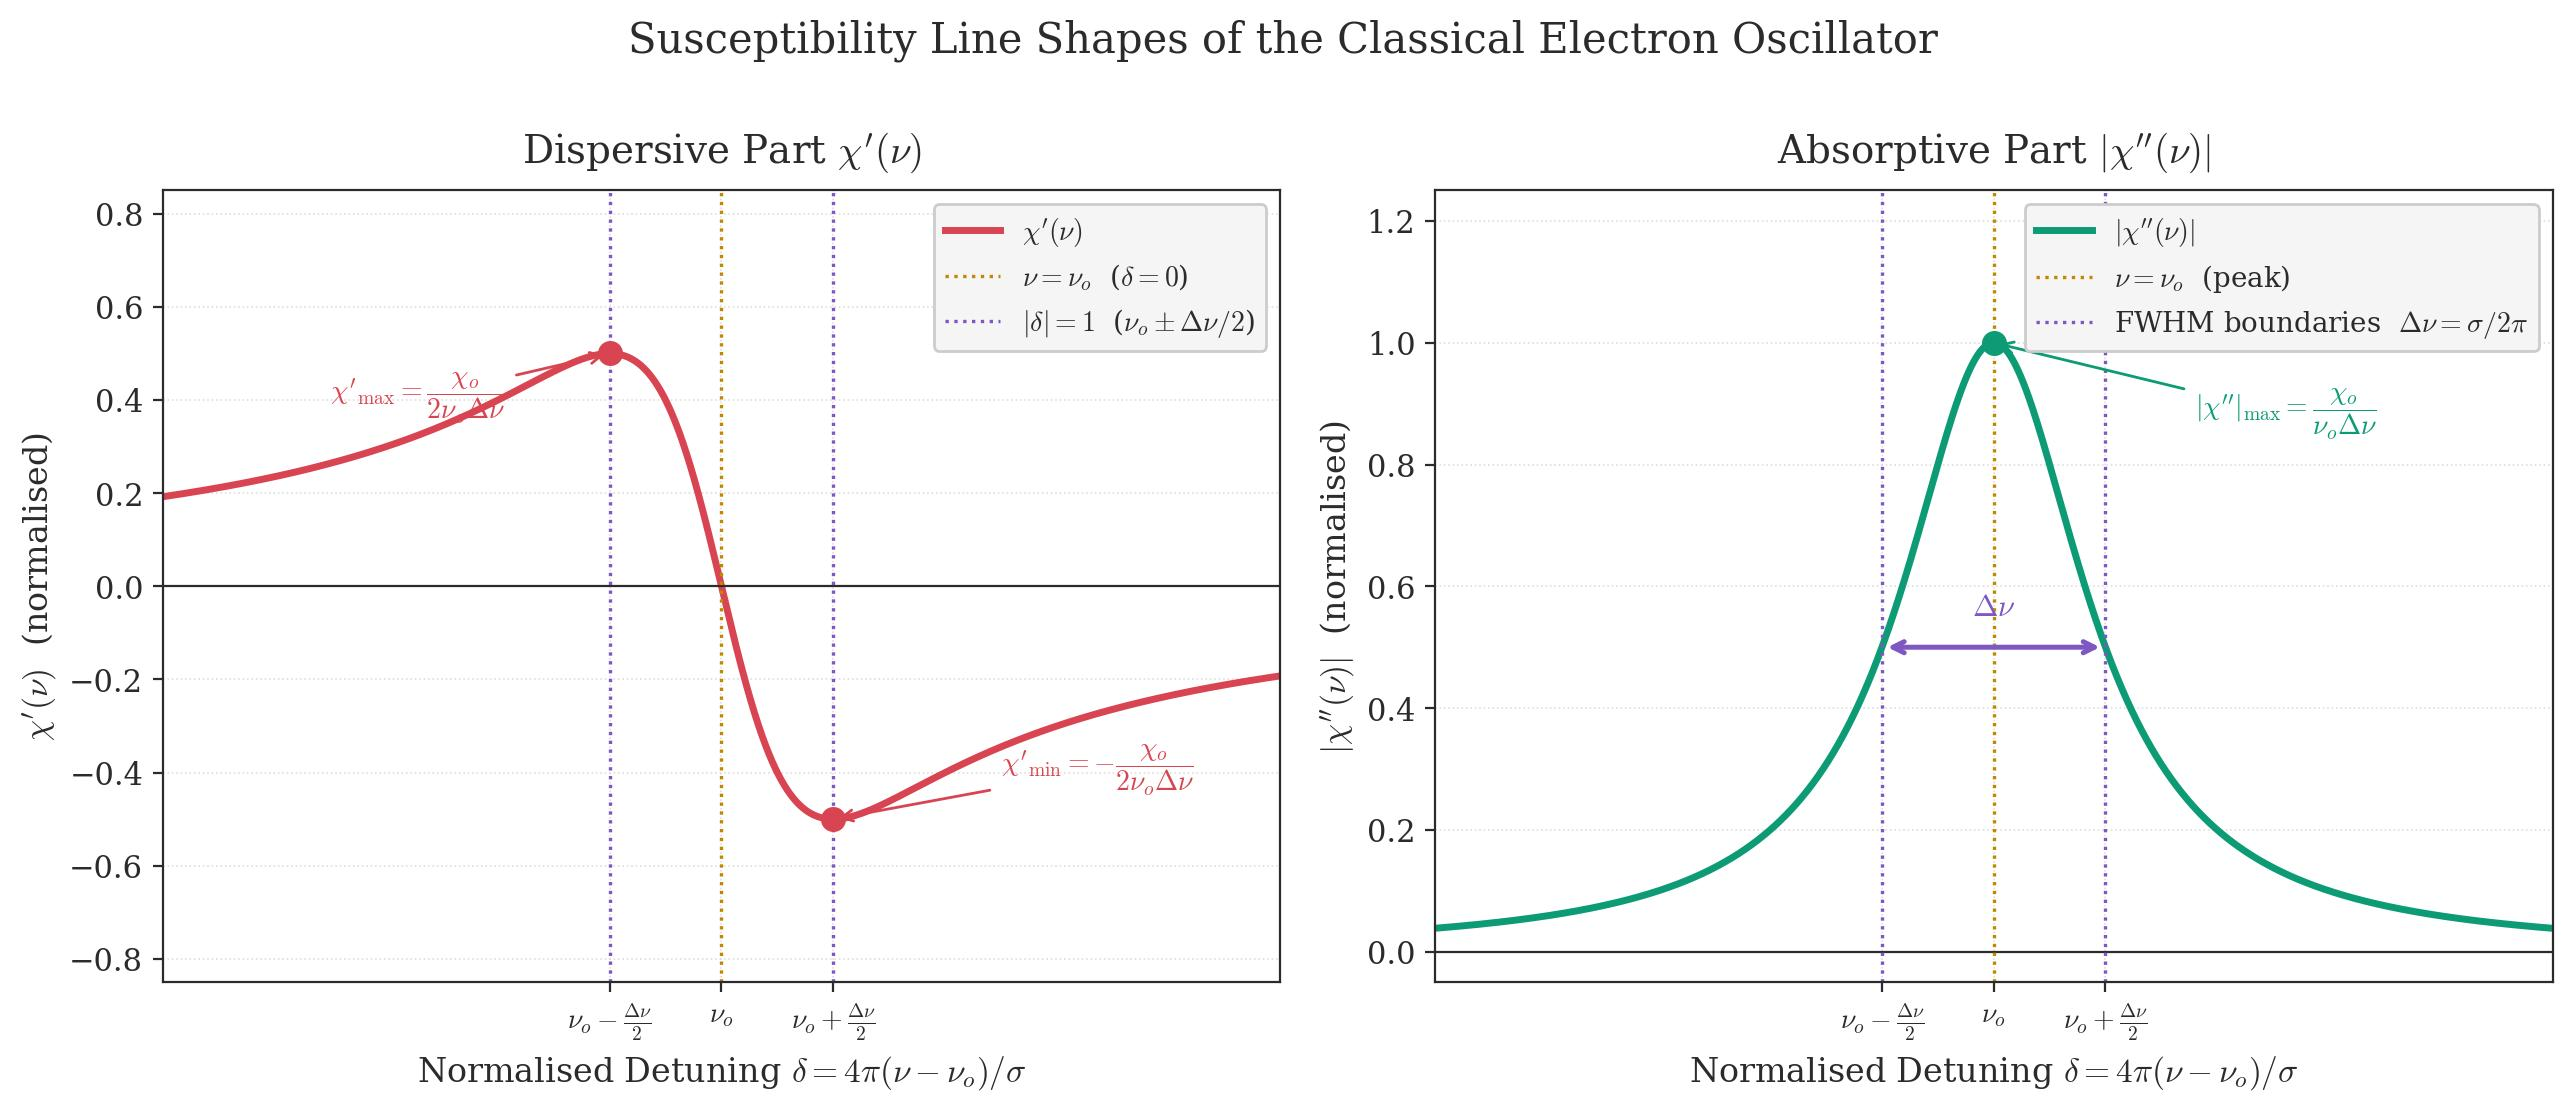
\includegraphics[width=0.95\textwidth]{../Figures/Sheet 1/q1d_susceptibility.jpg}
  \caption{Left: the dispersive real part $\chi'(\nu)$ with its extrema at $\nu_o \pm \Delta\nu/2$.
           Right: the absorptive imaginary part $|\chi''(\nu)|$ with its peak at $\nu_o$ and FWHM equal to $\Delta\nu$.}
\end{figure}

\medskip
\textbf{Part (E): Extremes of the relative permittivity $\epsilon_r$.}

The relative permittivity is $\epsilon_r(\nu) = 1 + \chi(\nu) = \epsilon_r'(\nu) + j\epsilon_r''(\nu)$, so directly:

\begin{equation*}
  \epsilon_r'(\nu) = 1 + \chi'(\nu) = 1 - \frac{\chi_o}{\nu_o\,\Delta\nu}\cdot\frac{\delta}{1+\delta^2},
  \qquad
  \epsilon_r''(\nu) = \chi''(\nu) = -\frac{\chi_o}{\nu_o\,\Delta\nu}\cdot\frac{1}{1+\delta^2}.
\end{equation*}

The extremes of $\epsilon_r'$ occur at the same $\delta = \pm 1$ as $\chi'$, giving

\begin{equation*}
  \boxed{\epsilon_r'(\nu)_{\max} = 1 + \frac{\chi_o}{2\nu_o\,\Delta\nu}, \qquad
  \epsilon_r'(\nu)_{\min} = 1 - \frac{\chi_o}{2\nu_o\,\Delta\nu}.}
\end{equation*}

For the limits: as $\nu \to \infty$, $\delta \to +\infty$, and both $\delta/(1+\delta^2)$ and $1/(1+\delta^2)$ vanish, so $\epsilon_r'(\nu) \to 1$ and $\epsilon_r''(\nu) \to 0$. As $\nu \to 0$, $\delta \to -2\nu_o/\Delta\nu \to -\infty$ (since $\nu_o \gg \Delta\nu$), so again both terms vanish and $\epsilon_r'(\nu) \to 1$, $\epsilon_r''(\nu) \to 0$.

The maximum magnitude of $\epsilon_r''$ occurs at resonance ($\delta = 0$):

\begin{equation*}
  \boxed{|\epsilon_r''(\nu_o)| = \frac{\chi_o}{\nu_o\,\Delta\nu}.}
\end{equation*}

\medskip
\textbf{Part (F): Finding $n'$ and $n''$ from $\epsilon_r$.}

The complex refractive index is defined by $n = n' + jn''= \sqrt{\epsilon_r}$. For a weak susceptibility ($\chi', \chi'' \ll 1$), we can Taylor-expand the square root:

\begin{equation*}
  n' + jn'' = \sqrt{1 + \chi' + j\chi''} \approx 1 + \frac{\chi' + j\chi''}{2},
\end{equation*}

separating real and imaginary parts immediately:

\begin{equation*}
  \boxed{n' = 1 + \frac{\chi'}{2}}
\end{equation*}
\begin{equation*}
  \boxed{n'' = \frac{\chi''}{2}.}
\end{equation*}

So the real part of the refractive index tracks the dispersive lineshape $\chi'$, while the imaginary part — which governs absorption — tracks the absorptive lineshape $\chi''$. The two are inseparably linked: wherever there is absorption there is also dispersion, and vice versa.

% ============================================================================

\begin{question}[Question 2]A non-absorptive medium of refractive index $n_{o}$ is host to impurities
with susceptibility $\chi=\chi'+j\chi''$. Show that the refractive index and power absorption
coefficient are given by
\begin{equation*}
  n = \sqrt{\frac{n_{o}^{2}+\chi'}{2}
      + \sqrt{\left(\frac{n_{o}^{2}+\chi'}{2}\right)^{2}+\left(\frac{\chi''}{2}\right)^{2}}}
  \qquad\mathrm{and}\qquad
  \alpha = -\frac{k_{o}}{n}\,\chi''.
\end{equation*}
Show that when $\chi'\ll 1$ and $\chi''\ll 1$, they reduce to
\begin{equation*}
  n\cong n_{o}+\frac{\chi'}{2n_{o}}
  \qquad\mathrm{and}\qquad
  \alpha\cong -\frac{k_{o}}{n_{o}}\,\chi''.
\end{equation*}
Find an expression for the range of frequencies at which $\partial n/\partial\omega<0$, i.e.\ the
medium is said to have an \emph{anomalous dispersion} as opposed to \emph{normal dispersion} at
which $\partial n/\partial\omega$ is positive.
\end{question}

\bigskip
\textbf{\large Solution --- Question 2}

\medskip
\textbf{Part 1: Deriving the exact expressions for $n$ and $\alpha$.}

A plane wave propagating through the medium carries a complex refractive index $\tilde{n} = n + jn_I$. Maxwell's equations dictate that $\tilde{n}^2 = \epsilon_r = n_o^2 + \chi' + j\chi''$. Expanding the square:

\begin{equation}
  (n + jn_I)^2 = n^2 - n_I^2 + 2jnn_I = n_o^2 + \chi' + j\chi''. \tag{I}
\end{equation}

Matching real and imaginary parts of \textup{(I)} separately:

\begin{equation*}
  n^2 - n_I^2 = n_o^2 + \chi', \qquad 2n\,n_I = \chi''.
\end{equation*}

From the second relation, $n_I = \chi''/(2n)$. Substituting into the first gives a quadratic in $n^2$:

\begin{equation*}
  n^2 - \frac{(\chi'')^2}{4n^2} = n_o^2 + \chi'
  \quad\Longrightarrow\quad
  n^4 - (n_o^2+\chi')\,n^2 - \frac{(\chi'')^2}{4} = 0.
\end{equation*}

Solving this as a quadratic in $n^2$ (taking the positive root, since $n^2 > 0$):

\begin{equation*}
  \boxed{n = \sqrt{\frac{n_o^2+\chi'}{2} + \sqrt{\!\left(\frac{n_o^2+\chi'}{2}\right)^{\!2}+\left(\frac{\chi''}{2}\right)^{\!2}}}}
\end{equation*}
\begin{equation*}
  \boxed{\alpha = -2n_I k_o = -\frac{k_o}{n}\,\chi''.}
\end{equation*}

where $k_o = \omega/c$ is the free-space wavenumber. The absorption coefficient emerges because the field amplitude decays as $e^{-n_I k_o z}$, so the intensity decays as $e^{-2n_I k_o z} = e^{-\alpha z}$. Since $\chi'' < 0$ for a passive medium, $\alpha > 0$ as expected.

\medskip
\textbf{Part 2: The weak-susceptibility limit ($\chi', \chi'' \ll 1$).}

When both susceptibility components are small compared to $n_o^2$, the inner square root in the expression for $n$ simplifies. We factor $(n_o^2 + \chi')/2$ out of the square root:

\begin{equation*}
  n \approx \sqrt{\frac{n_o^2+\chi'}{2} + \frac{n_o^2+\chi'}{2}
  \sqrt{1+\left(\frac{\chi''}{n_o^2+\chi'}\right)^{\!2}}}
  \approx \sqrt{n_o^2 + \chi'} = n_o\sqrt{1 + \frac{\chi'}{n_o^2}},
\end{equation*}

where we dropped the $(\chi'')^2$ term as second-order small. Taylor-expanding the remaining square root to first order:

\begin{equation*}
  \boxed{n \cong n_o + \frac{\chi'}{2n_o}.}
\end{equation*}

For the absorption coefficient, substituting $n \approx n_o$ into $n_I = \chi''/(2n)$:

\begin{equation*}
  n_I \approx \frac{\chi''}{2n_o},
  \qquad\Longrightarrow\qquad \alpha = -2n_I k_o \cong -\frac{k_o}{n_o}\,\chi''.
\end{equation*}

\medskip
\textbf{Part 3: The range of anomalous dispersion.}

Since $n \cong n_o + \chi'/(2n_o)$, we have $\partial n/\partial\omega \propto \partial\chi'/\partial\omega \propto \partial\chi'/\partial\nu \propto \partial\chi'/\partial\delta$. Differentiating $\chi'(\delta) \propto -\delta/(1+\delta^2)$ with respect to $\delta$:

\begin{equation*}
  \frac{\partial\chi'}{\partial\delta} \propto \frac{\delta^2 - 1}{(1+\delta^2)^2}.
\end{equation*}

This is negative when $\delta^2 < 1$, i.e.\ $-1 < \delta < 1$. Converting back to frequency using $\delta = 4\pi(\nu - \nu_o)/\sigma = 2(\nu-\nu_o)/\Delta\nu$:

\begin{equation*}
  \boxed{\frac{\partial n}{\partial\omega} < 0 \quad\Longleftrightarrow\quad
  \nu_o - \frac{\Delta\nu}{2} < \nu < \nu_o + \frac{\Delta\nu}{2}.}
\end{equation*}

Anomalous dispersion is confined to the absorption band itself — a frequency window of width $\Delta\nu$ centred on the resonance. Outside this window $\partial n/\partial\omega > 0$ everywhere, which is the normal dispersion that gives a glass prism its familiar rainbow.

% ============================================================================

\begin{question}[Question 3]The real and imaginary parts $\chi'$ and $\chi''$ of the susceptibility
$\chi$ are not independent. One cannot change without changing the other. For the CEO they are
related by $\chi'=2(\nu-\nu_{o})\chi''/\Delta\nu$. Propose a setup for measuring the refractive
index dispersion that utilises this relation.
\end{question}

\bigskip
\textbf{\large Solution --- Question 3}

\medskip
The key observation is that the relation $\chi' = 2(\nu-\nu_o)\chi''/\Delta\nu$ links the \emph{dispersive} part of the susceptibility (which determines the refractive index via $n \approx 1 + \chi'/2$) to the \emph{absorptive} part (which determines the absorption coefficient via $\alpha \propto -\chi''$). This means a single absorption measurement is sufficient to reconstruct the full refractive index dispersion curve --- no interferometer is needed.

\medskip
\textbf{Proposed experimental setup.}

Pass a broadband (or tunable) light source through a sample of length $L$ and record the transmitted intensity spectrum $I(\nu)$. From the Beer--Lambert law

\begin{equation*}
  I(\nu) = I_0(\nu)\,e^{-\alpha(\nu)L}
  \quad\Longrightarrow\quad
  \alpha(\nu) = -\frac{1}{L}\ln\!\left(\frac{I(\nu)}{I_0(\nu)}\right),
\end{equation*}

where $I_0(\nu)$ is a reference spectrum recorded without the sample. Since $\alpha = -k_o\chi''/n_o \approx -k_o\chi''$ (for weak absorption), we extract

\begin{equation*}
  \chi''(\nu) \approx -\frac{n_o\,\alpha(\nu)}{k_o}.
\end{equation*}

Applying the given relation immediately yields the dispersive part:

\begin{equation*}
  \boxed{\chi'(\nu) = \frac{2(\nu-\nu_o)}{\Delta\nu}\,\chi''(\nu)}
  \quad\Longrightarrow\quad
  n(\nu) \approx n_o + \frac{\chi'(\nu)}{2n_o}.
\end{equation*}

Physically, this works because the real and imaginary parts of any causal response function are related by the Kramers--Kronig relations. The CEO expression $\chi' = 2(\nu-\nu_o)\chi''/\Delta\nu$ is the near-resonance approximation of the full Kramers--Kronig integral. The practical advantage is significant: absorption spectroscopy is straightforward and does not require the phase-sensitive measurements (e.g.\ interferometry or ellipsometry) that a direct determination of $n(\nu)$ would otherwise demand.

% ============================================================================

\begin{question}[Question 4]Solid materials that could be used for making optical fibres typically
exhibit strong absorption in the blue or ultraviolet region and strong absorption in the middle
infrared region. Modelling the material as having two narrow resonant absorptions at wavelengths
$\lambda_{01}$ and $\lambda_{02}$, sketch the wavelength dependence of the refractive index.
Assume that the parameter $\chi_{o}$ is the same for both resonances.
\end{question}

\bigskip
\textbf{\large Solution --- Question 4}

\medskip
The refractive index of a medium with a single resonance follows the dispersive lineshape $n(\nu) \approx n_o + \chi'(\nu)/(2n_o)$, which rises just below the resonance, passes through a local maximum, then dips sharply through $n_o$ at the resonance centre $\nu_o$, reaches a local minimum just above it, and slowly recovers back to $n_o$ far from resonance. For an optical-fibre material with two resonances — one at $\nu_{01}$ in the ultraviolet/blue and one at $\nu_{02}$ in the mid-infrared — the total $\chi'$ is the sum of two such dispersive contributions. The refractive index is plotted below.

\begin{figure}[H]
  \centering
  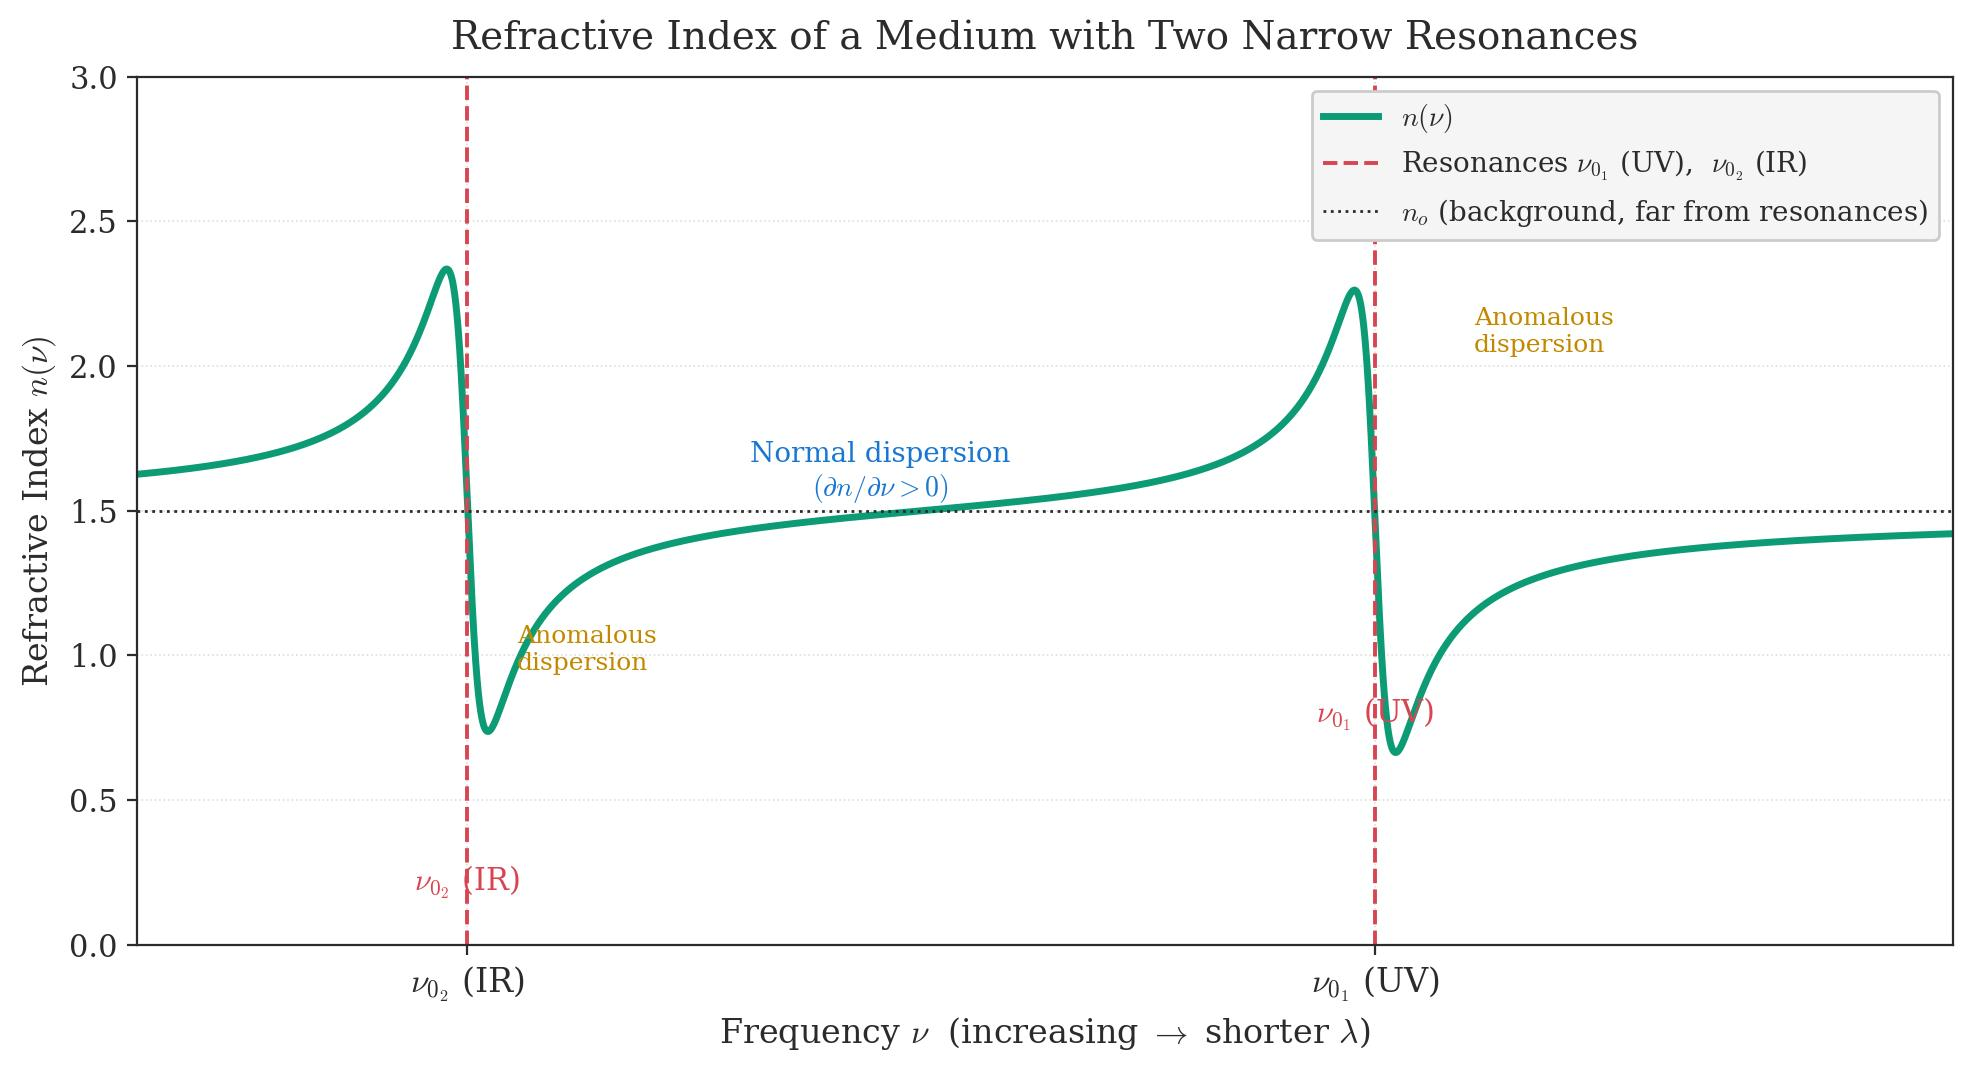
\includegraphics[width=0.88\textwidth]{../Figures/Sheet 1/q4_refractive_index_two_res.jpg}
  \caption{Wavelength (frequency) dependence of the refractive index for a medium with two
           narrow resonances at $\nu_{01}$ (UV) and $\nu_{02}$ (IR).  Between the resonances the
           medium exhibits normal dispersion ($\partial n/\partial\nu > 0$); inside each
           absorption band the dispersion is anomalous.  Far from both resonances $n\to n_o$.}
\end{figure}

Between the two resonances — spanning the visible range for a typical silica fibre — both contributions to $\chi'$ add constructively on their respective low-frequency tails, so the background index is elevated above $n_o$ and increases with frequency (normal dispersion). Near each resonance the dispersive swing causes anomalous dispersion within a bandwidth $\Delta\nu$. The asymptotic level far below $\nu_{02}$ and far above $\nu_{01}$ returns to $n_o$ in both cases, since $\chi' \to 0$ as $|\delta| \to \infty$.

% ============================================================================

\begin{question}[Question 5]Consider the CEO model for the case in which there is no field acting on
the atom. Suppose that at $t=0$ an electron is given the displacement $x_{o}$ from equilibrium
and the velocity $v_{o}$.

\begin{enumerate}[label=(\alph*)]
  \item Show that in the lossless case the electron coordinate $x(t)$ is given by
        \begin{equation*}
          x(t)=x_{o}\cos\omega_{o}t+\frac{v_{o}}{\omega_{o}}\sin\omega_{o}t.
        \end{equation*}
  \item What is the total (kinetic plus potential) energy of the electron in this case?

  \item If the radiated power corresponds to a radiation force
        $F_{\mathrm{rad}}/m=\dfrac{\gamma_{r}}{m\omega_{o}^{2}}\,\dfrac{\partial^{3}x}{\partial t^{3}}$,
        where $\gamma_{r}=q^{2}\omega_{o}^{2}/6\pi\epsilon_{o}c^{3}$, then show that the
        electron is expected to radiate away most of its energy in a time
        \begin{equation*}
          \tau_{r}=4\pi\epsilon_{o}\!\left(\frac{3mc^{3}}{2e^{2}\omega_{o}^{2}}\right).
        \end{equation*}
        This is the classical picture of ``spontaneous emission'' which we will later consider
        during our study in the course.

        \emph{Hint:} Use a trial solution $x(t)=e^{st}$, with $s=j\omega_{o}+\eta$ and show
        that $\eta\approx\gamma_{r}/2$.

  \item Estimate numerically the ``radiative lifetime'' $\tau_{r}$ found in part (c) for the
        case of an electron oscillating at an optical frequency $\nu_{o}(=\omega_{o}/2\pi)$.
\end{enumerate}
\end{question}

\bigskip
\textbf{\large Solution --- Question 5}

\medskip
\textbf{Part (a): Lossless free oscillation.}

With no external field and no damping, the equation of motion reduces to the simple harmonic oscillator:

\begin{equation*}
  \frac{\partial^2 x}{\partial t^2} + \omega_o^2\,x(t) = 0.
\end{equation*}

The general solution is $x(t) = C e^{j\omega_o t} + D e^{-j\omega_o t}$, which we rewrite as real sinusoids: $x(t) = A\cos(\omega_o t) + B\sin(\omega_o t)$. Applying the initial conditions:

\begin{equation*}
  x(0) = A = x_o, \qquad
  \dot{x}(0) = B\omega_o = v_o \;\Longrightarrow\; B = \frac{v_o}{\omega_o}.
\end{equation*}

\begin{equation*}
  \boxed{x(t) = x_o\cos(\omega_o t) + \frac{v_o}{\omega_o}\sin(\omega_o t).}
\end{equation*}

\medskip
\textbf{Part (b): Total mechanical energy.}

The total energy is the sum of potential energy $\tfrac{1}{2}kx^2 = \tfrac{1}{2}m\omega_o^2 x^2$ and kinetic energy $\tfrac{1}{2}m\dot{x}^2$. Since the system is lossless, energy is conserved and we simply evaluate at $t=0$:

\begin{equation*}
  \boxed{U = \tfrac{1}{2}m\omega_o^2 x_o^2 + \tfrac{1}{2}m v_o^2.}
\end{equation*}

One can verify this by computing $U(t)$ explicitly — the cross terms cancel via the Pythagorean identity $\cos^2 + \sin^2 = 1$, confirming $U(t) = U(0)$ for all $t$.

\medskip
\textbf{Part (c): Radiative lifetime $\tau_r$.}

Including the radiation reaction force, the equation of motion becomes

\begin{equation*}
  \frac{\partial^2 x}{\partial t^2} + \omega_o^2\,x = \frac{F_{\mathrm{rad}}}{m}
  = \frac{\gamma_r}{m\omega_o^2}\,\frac{\partial^3 x}{\partial t^3}.
\end{equation*}

Rearranging so all terms are on the same side:

\begin{equation*}
  -\frac{\gamma_r}{m\omega_o^2}\,\frac{\partial^3 x}{\partial t^3}
  + \frac{\partial^2 x}{\partial t^2} + \omega_o^2\,x = 0.
\end{equation*}

Substituting the trial solution $x(t) = e^{st}$ with $s = j\omega_o + \eta$, each derivative contributes a factor of $s$:

\begin{equation*}
  -\frac{\gamma_r}{m\omega_o^2}\,s^3 + s^2 + \omega_o^2 = 0.
\end{equation*}

Now we use the key observation: since $s^2 = (j\omega_o + \eta)^2 \approx -\omega_o^2$ for $|\eta| \ll \omega_o$, we have $s^3 = s \cdot s^2 \approx s(-\omega_o^2)$. Substituting this approximation:

\begin{equation*}
  -\frac{\gamma_r}{m\omega_o^2}\cdot(-\omega_o^2)\,s + s^2 + \omega_o^2 = 0
  \quad\Longrightarrow\quad
  s^2 + \frac{\gamma_r}{m}\,s + \omega_o^2 = 0.
\end{equation*}

Solving this quadratic:

\begin{equation*}
  s = -\frac{\gamma_r}{2m} \pm \sqrt{\left(\frac{\gamma_r}{2m}\right)^{\!2} - \omega_o^2}
  \approx -\frac{\gamma_r}{2m} \pm j\omega_o,
\end{equation*}

where the square root is approximated by $j\omega_o$ since $\gamma_r/(2m) \ll \omega_o$. Comparing with the assumed form $s = j\omega_o + \eta$, we identify:

\begin{equation*}
  \eta = -\frac{\gamma_r}{2m}.
\end{equation*}

The amplitude decays as $e^{\eta t} = e^{-\gamma_r t/(2m)}$, so the energy (proportional to amplitude squared) decays as $e^{-\gamma_r t/m}$. The electron radiates away most of its energy in a time $\tau_r = m/\eta_{\text{rate}} = 2m/\gamma_r$. Substituting $\gamma_r = q^2\omega_o^2/(6\pi\epsilon_o c^3)$ with $q = e$:

\begin{equation*}
  \tau_r = \frac{2m}{\gamma_r} = \frac{2m \cdot 6\pi\epsilon_o c^3}{e^2\omega_o^2}
  = \frac{12\pi\epsilon_o m c^3}{e^2\omega_o^2}.
\end{equation*}

Writing $12\pi = 4\pi \cdot 3$ and grouping:

\begin{equation*}
  \boxed{\tau_r = 4\pi\epsilon_o\!\left(\frac{3mc^3}{2e^2\omega_o^2}\right).}
\end{equation*}

Physically, $\tau_r$ is the classical radiative lifetime — the time a freely oscillating electron takes to radiate away its stored mechanical energy. It is the classical precursor to the concept of spontaneous emission lifetime that quantum mechanics later derives rigorously.

\medskip
\textbf{Part (d): Numerical estimate of $\tau_r$ at an optical frequency.}

Taking a representative optical frequency $\nu_o \approx 5\times10^{14}$\,Hz (green light, $\lambda \approx 600$\,nm), the angular frequency is $\omega_o = 2\pi\nu_o \approx 3.14\times10^{15}$\,rad/s. Substituting into the formula from part (c) with $e = 1.602\times10^{-19}$\,C, $m = 9.109\times10^{-31}$\,kg, $c = 3\times10^8$\,m/s, $\epsilon_o = 8.854\times10^{-12}$\,F/m:

\begin{equation*}
  \tau_r = 4\pi\epsilon_o\!\left(\frac{3mc^3}{2e^2\omega_o^2}\right)
  \approx \frac{4\pi\times8.854\times10^{-12}\times 3\times9.109\times10^{-31}\times(3\times10^8)^3}{2\times(1.602\times10^{-19})^2\times(3.14\times10^{15})^2}.
\end{equation*}

Evaluating numerator and denominator separately:

\begin{equation*}
  \text{Num.} \approx 8.21\times10^{-15}, \qquad
  \text{Den.} \approx 5.06\times10^{-7},
\end{equation*}

\begin{equation*}
  \boxed{\tau_r \approx 1.6\times10^{-8}\,\text{s} = 16\,\text{ns}.}
\end{equation*}

This is the classical prediction for how long it takes a free electron oscillating at optical frequencies to radiate away its energy. Interestingly, real atoms (e.g.\ the hydrogen $2p$ state, $\tau \approx 1.6$\,ns) radiate roughly an order of magnitude faster because quantum mechanics introduces factors such as transition matrix elements that the purely classical model cannot capture.

% ============================================================================

\begin{question}[Question 6]Consider the case of a single loop RLC circuit with no voltage or current
source. Find the transient solution of the charge of the capacitance. Then assume that a
sinusoidal voltage source is connected in series with the loop elements. Write down the equation
of the charge of the capacitance and find its solution. What is the analogy of the inductance,
capacitance, and resistance of the CEO model of an atom subjected to external radiation?
\end{question}

\bigskip
\textbf{\large Solution --- Question 6}

\medskip
\textbf{Transient response (no source).}

For a series LRC loop the Kirchhoff voltage relation reads $V = LQ'' + RQ' + Q/C$, where $Q$ is the charge on the capacitor and primes denote time derivatives. Dividing through by $L$ and defining

\begin{equation*}
  \eta \equiv \frac{R}{L}, \qquad \omega_o^2 \equiv \frac{1}{LC},
\end{equation*}

the equation becomes $Q'' + \eta Q' + \omega_o^2 Q = V/L$. With no source ($V=0$) we substitute the trial $Q \propto e^{st}$:

\begin{equation*}
  s^2 + \eta s + \omega_o^2 = 0
  \quad\Longrightarrow\quad
  s = -\frac{\eta}{2} \pm \sqrt{\left(\frac{\eta}{2}\right)^{\!2} - \omega_o^2}.
\end{equation*}

In the underdamped case $\omega_o > \eta/2$, the square root is imaginary. Defining the damped frequency $\omega_d = \sqrt{\omega_o^2 - (\eta/2)^2}$, the general transient solution is

\begin{equation*}
  \boxed{Q(t) = Q_o\,e^{-\eta t/2}\cos(\omega_d t + \theta).}
\end{equation*}

The charge on the capacitor therefore oscillates at the damped frequency $\omega_d$ while its amplitude decays exponentially with time constant $2/\eta = 2L/R$. Larger resistance drains energy faster and shortens the transient.

\medskip
\textbf{Forced (sinusoidal source) response.}

Assume $V(t) = \mathrm{Re}[V_o\,e^{j(\omega t+\theta)}]$ and seek $Q(t) = \mathrm{Re}[Q_o\,e^{j(\omega t+\theta)}]$. Substituting into $L Q'' + R Q' + Q/C = V$ and cancelling the common exponential:

\begin{equation*}
  \frac{V_o}{L} = Q_o\bigl(-\omega^2 + j\omega\eta + \omega_o^2\bigr)
  \quad\Longrightarrow\quad
  Q_o = \frac{V_o/L}{\omega_o^2 - \omega^2 + j\omega\eta},
\end{equation*}

so the physical charge is

\begin{equation*}
  \boxed{Q(t) = \mathrm{Re}\!\left[\frac{V_o/L}{\omega_o^2 - \omega^2 + j\omega\eta}\,e^{j(\omega t+\theta)}\right].}
\end{equation*}

This is formally identical to the CEO polarisation amplitude: the denominator $\omega_o^2 - \omega^2 + j\omega\eta$ is the Lorentzian resonance denominator we derived in Question 1.

\medskip
\textbf{CEO analogy.}

Comparing the LRC equation $LQ'' + RQ' + (1/C)Q = V$ with the CEO equation $m\ddot{x} + b\dot{x} + kx = -eE$ (where $b = m\sigma$ is the damping coefficient) term by term:

\begin{center}
\begin{tabular}{cc}
  \toprule
  \textbf{LRC circuit} & \textbf{CEO model} \\
  \midrule
  Inductance $L$ & Electron mass $m$ \\
  Resistance $R$ & Damping coefficient $b = m\sigma$ \\
  Compliance $C$ & Inverse spring constant $1/k$ \\
  \bottomrule
\end{tabular}
\end{center}

The voltage $V$ driving the circuit maps to the force $-eE$ driving the electron, and the charge $Q$ maps to the displacement $x$. The resonance frequency $\omega_o = 1/\sqrt{LC}$ of the circuit maps exactly to $\omega_o = \sqrt{k/m}$ of the oscillator.

% ============================================================================

\begin{question}[Question 7]Suppose that the electron in the Lorentz model rotates in a stationary
orbit of radius $R_{o}$ with a uniform speed $V$ subject to an internal electric field $E_{o}$
due to the nucleus. The electric field $E$ due to external radiation displaces the electron in
the radial direction (i.e.\ changes its orbit radius) by a displacement $x$.

\begin{enumerate}[label=(\arabic*)]
  \item Show that
        $x/R_{o}=E/E_{o}+(E/E_{o})^{2}+(E/E_{o})^{3}+\cdots$
  \item If $R_{o}=1.0\,\text{\AA}$, then estimate the value of $E_{o}$ and the coefficients of
        the quadratic and cubic terms in the relation between $x$ and $E$. Hence find the
        condition under which this relation is linear as assumed in the Lorentz model. Show that
        in the case of a linear relation the force acting on the electron due to the external
        field follows Hooke's law. Then find an expression of the spring constant and estimate
        its value and the value of the resonance frequency.
\end{enumerate}

Answer the following two questions:
\begin{enumerate}[label=Q(\arabic*)]
  \item In which range of the electromagnetic spectrum does the resonance frequency lie?
  \item When do you expect linearity to apply or not apply?
\end{enumerate}
\end{question}

\bigskip
\textbf{\large Solution --- Question 7}

\medskip
\textbf{Part (1): Deriving the displacement series.}

Before any external radiation, the electron moves in a circular orbit of radius $R_o$ at speed $V$. Radial force balance between the electrostatic attraction $eE_o$ and the centripetal acceleration gives:

\begin{equation*}
  -eE_o + \frac{mV^2}{R_o} = 0 \quad\Longrightarrow\quad mV^2 = eE_oR_o. \tag{i}
\end{equation*}

When the external field $E$ is applied radially, it displaces the electron to a new orbit radius $R_o + x$. The orbital speed $V$ is unchanged (the field acts only radially on the instantaneous position), so the new force balance is:

\begin{equation*}
  -eE_o + \frac{mV^2}{R_o + x} = -eE.
\end{equation*}

Substituting $mV^2 = eE_oR_o$ from (i):

\begin{equation*}
  -eE_o + \frac{eE_oR_o}{R_o + x} = -eE
  \quad\Longrightarrow\quad
  1 = \frac{R_o}{R_o + x} + \frac{E}{E_o}
  \quad\Longrightarrow\quad
  \frac{1}{1 + x/R_o} = 1 - \frac{E}{E_o}.
\end{equation*}

Taking the reciprocal and using the geometric series $1/(1-u) = 1 + u + u^2 + \cdots$ valid for $u = E/E_o < 1$:

\begin{equation*}
  1 + \frac{x}{R_o} = \frac{1}{1 - E/E_o} = 1 + \frac{E}{E_o} + \left(\frac{E}{E_o}\right)^{\!2} + \left(\frac{E}{E_o}\right)^{\!3} + \cdots
\end{equation*}

\begin{equation*}
  \boxed{\frac{x}{R_o} = \frac{E}{E_o} + \left(\frac{E}{E_o}\right)^{\!2} + \left(\frac{E}{E_o}\right)^{\!3} + \cdots \qquad (E < E_o).}
\end{equation*}

\medskip
\textbf{Part (2): Numerical values for $R_o = 1\,\text{\AA}$.}

The internal field $E_o$ is the Coulomb field at distance $R_o$ from the nucleus ($Z=1$):

\begin{equation*}
  E_o = \frac{e}{4\pi\epsilon_o R_o^2}
  = \frac{1.602\times10^{-19}}{4\pi\times8.854\times10^{-12}\times(10^{-10})^2}
  \approx 144\,\text{GV/m}.
\end{equation*}

The series coefficients for the displacement $x = R_o(E/E_o + \cdots)$ expressed in $x$ vs.\ $E$ are:

\begin{equation*}
  \text{Linear:}\quad \frac{R_o}{E_o} = \frac{1}{E_o} \approx 7\,\text{pm/V} = 7\times10^{-12}\,\text{m/V},
\end{equation*}
\begin{equation*}
  \text{Quadratic:}\quad \frac{R_o}{E_o^2} = \frac{1}{E_o^2} \approx 49\times10^{-24}\,(\text{m/V})^2,
\end{equation*}
\begin{equation*}
  \text{Cubic:}\quad \frac{R_o}{E_o^3} = \frac{1}{E_o^3} \approx 343\times10^{-36}\,(\text{m/V})^3.
\end{equation*}

\textbf{Linearity condition.} The relation becomes effectively linear when the quadratic term is negligible compared to the linear term, i.e.\ $(E/E_o)^2 \ll E/E_o$, giving:

\begin{equation*}
  \boxed{E \ll E_o \approx 144\,\text{GV/m}.}
\end{equation*}

\textbf{Hooke's law.} In the linear limit $x \approx R_oE/E_o$, so $E = E_ox/R_o$. The force on the electron due to the external field is:

\begin{equation*}
  F_{E_{\mathrm{ext}}} = -eE = -\frac{eE_o}{R_o}\,x = -k_x x,
\end{equation*}

which is exactly Hooke's law with spring constant:

\begin{equation*}
  k_x = \frac{eE_o}{R_o} = \frac{e^2}{4\pi\epsilon_o R_o^3}
  = \frac{(1.602\times10^{-19})^2}{4\pi\times8.854\times10^{-12}\times(10^{-10})^3}
  \approx 230.7\,\text{N/m}.
\end{equation*}

The resonance (natural) frequency of this spring-electron system is then:

\begin{equation*}
  \omega_o = \sqrt{\frac{k_x}{m}}
  = \sqrt{\frac{e^2}{4\pi\epsilon_o R_o^3 m}}
  \approx \sqrt{\frac{230.7}{9.109\times10^{-31}}}
  \approx 1.59\times10^{16}\,\text{rad/s},
\end{equation*}
\begin{equation*}
  \boxed{f_o = \frac{\omega_o}{2\pi} \approx 2.5\times10^{15}\,\text{Hz}.}
\end{equation*}

\medskip
\textbf{Q(1): Spectral range of $f_o$.} With $\lambda_o = c/f_o \approx 120$\,nm, the resonance lies in the \emph{ultraviolet/optical} region of the electromagnetic spectrum --- consistent with the fact that electronic resonances of atoms are typically in the UV-visible range.

\textbf{Q(2): When does linearity apply or break down?} Linearity holds whenever the applied radiation field satisfies $E \ll E_o \approx 144$\,GV/m. For conventional optical sources this condition is comfortably met, justifying the linear Lorentz model. It breaks down only at extreme laser intensities (focused ultrashort pulses reaching $\sim10^{10}$\,W/cm$^2$ and above), where $E$ becomes comparable to $E_o$ and higher-order terms in the displacement series become significant --- the regime of \emph{nonlinear optics}.

% ============================================================================

\begin{question}[Bonus Question]In the CEO model introduced in lectures the nucleus is assumed to be so
massive compared to an electron that its acceleration is generally negligible (compare between the
mass of a proton and an electron). Suppose that this assumption is not applied. Show that the CEO
model still applies provided that the electron mass is replaced with the \emph{reduced mass} and
that no change takes place in the momentum of the atom.
\end{question}

\bigskip
\textbf{\large Solution --- Bonus Question}

\medskip
The standard CEO derivation fixes the nucleus and writes the equation of motion only for the electron. We now allow both particles to move and track two coordinates: $x_e$ for the electron and $x_n$ for the nucleus. The internal restoring force depends on their \emph{relative} displacement $x = x_e - x_n$, and each particle is driven by the external field according to its charge.

\medskip
\textbf{Equations of motion for each particle.}

Electron (charge $-e$, mass $m_e$):

\begin{equation*}
  m_e\,\ddot{x}_e = -k(x_e - x_n) - b(\dot{x}_e - \dot{x}_n) - eE.
\end{equation*}

Nucleus (charge $+e$, mass $m_n$):

\begin{equation*}
  m_n\,\ddot{x}_n = +k(x_e - x_n) + b(\dot{x}_e - \dot{x}_n) + eE.
\end{equation*}

\medskip
\textbf{Centre-of-mass momentum is conserved.}

Adding the two equations cancels every internal force:

\begin{equation*}
  m_e\,\ddot{x}_e + m_n\,\ddot{x}_n = (-eE) + (+eE) = 0
  \quad\Longrightarrow\quad
  \frac{d}{dt}\bigl(m_e\dot{x}_e + m_n\dot{x}_n\bigr) = 0.
\end{equation*}

The total momentum of the atom is constant because the net charge is zero: the forces the field exerts on the electron and nucleus are equal in magnitude and opposite in sign, and they cancel exactly. No net momentum is imparted to the atom.

\medskip
\textbf{Equation of motion for the relative coordinate.}

Divide each equation by its mass and subtract:

\begin{equation*}
  \ddot{x}_e - \ddot{x}_n = -\frac{k}{\mu}\,x - \frac{b}{\mu}\,\dot{x} - \frac{e}{\mu}\,E,
  \qquad \frac{1}{\mu} \equiv \frac{1}{m_e} + \frac{1}{m_n},
\end{equation*}

where $\mu = m_e m_n/(m_e + m_n)$ is the \emph{reduced mass}. Writing $\ddot{x} = \ddot{x}_e - \ddot{x}_n$:

\begin{equation*}
  \boxed{\mu\,\ddot{x} + b\,\dot{x} + k\,x = -eE.}
\end{equation*}

This is identical to the original CEO equation with $m_e \to \mu$. Every subsequent result --- susceptibility, linewidth, refractive index --- carries over with this single substitution. Since $m_n \gg m_e$, the reduced mass satisfies $\mu \approx m_e$, confirming that the fixed-nucleus approximation is excellent in practice.

% ============================================================================

\begin{question}[Formative Question]What changes should be made to the CEO model in the case
of conductors where at room temperature valence electrons are free to move away from their mother
atoms? Derive an expression of the electron susceptibility and dielectric constant in this case.
\end{question}

\bigskip
\textbf{\large Solution --- Formative Question}

\medskip
In a conductor, valence electrons are \emph{free}: there is no restoring spring, so $k = 0$ and hence $\omega_o = 0$. The CEO equation of motion reduces to:

\begin{equation*}
  m\,\ddot{x} + m\sigma\,\dot{x} = -eE.
\end{equation*}

Substituting the phasor $x(t) = \mathrm{Re}[x(\omega)\,e^{j\omega t}]$:

\begin{equation*}
  m(-\omega^2 + j\sigma\omega)\,x = -eE
  \quad\Longrightarrow\quad
  x(\omega) = \frac{eE}{m(\omega^2 - j\sigma\omega)}.
\end{equation*}

\medskip
\textbf{Susceptibility of the free-electron gas.}

The polarisation is $P = -Nex$ and $\chi = P/(\epsilon_o E)$:

\begin{equation*}
  \chi(\omega) = -\frac{Ne^2}{m\epsilon_o(\omega^2 - j\sigma\omega)}
  = -\frac{\omega_p^2}{\omega^2 - j\sigma\omega},
\end{equation*}

where the \emph{plasma frequency} is defined by

\begin{equation*}
  \boxed{\omega_p = \sqrt{\frac{Ne^2}{m\epsilon_o}}.}
\end{equation*}

\medskip
\textbf{Relative permittivity (Drude model).}

The dielectric constant is:

\begin{equation*}
  \boxed{\epsilon_r(\omega) = 1 + \chi = 1 - \frac{\omega_p^2}{\omega^2 - j\sigma\omega}.}
\end{equation*}

In the lossless limit $\sigma \to 0$: $\epsilon_r = 1 - \omega_p^2/\omega^2$. Two regimes follow directly:

\begin{itemize}
  \item $\omega > \omega_p$: $\epsilon_r > 0 \Rightarrow n$ is real --- the conductor is \emph{transparent}.
  \item $\omega < \omega_p$: $\epsilon_r < 0 \Rightarrow n$ is purely imaginary --- waves are evanescent and the metal is \emph{opaque and highly reflective}.
\end{itemize}

The free-electron result is recovered from the bound-electron CEO simply by setting $\omega_o = 0$: the resonance ``slides'' to zero frequency, the restoring spring disappears, and the dispersive Lorentzian shape is replaced by the $1/\omega^2$ Drude roll-off.
